\documentclass[british]{beamer}
\usepackage{pgfpages}

\mode<presentation>
\usetheme{Berlin}
\usecolortheme{beaver}
%\setbeameroption{show notes on second screen=right}
\beamertemplatenavigationsymbolsempty
\setbeamercovered{transparent}

\usepackage{graphicx}
\usepackage{amsmath}
\usepackage{amssymb}
\usepackage{amsfonts}
\usepackage{tikz}
\usepackage{pgfplots}
\usepackage{pgfplotstable}
\usepackage{booktabs}
\usepackage{fontspec}
\usepackage{babel}
\usepackage{url}
\usepackage{csquotes}
\usepackage{xcolor}
\usepackage{units}
\usepackage{siunitx}
\usepackage[backend=biber,style=authoryear,maxcitenames=2]{biblatex}

\addbibresource{../bibliography/strings.bib}
\addbibresource{../bibliography/citations.bib}
\addbibresource{../bibliography/linguistics.bib}

% workaround for invisible text when using notes (https://tex.stackexchange.com/a/306662)
\makeatletter 
\def\beamer@framenotesbegin{% at beginning of slide
     \usebeamercolor[fg]{normal text}
      \gdef\beamer@noteitems{}% 
      \gdef\beamer@notes{}% 
}
\makeatother

%\newfontfamily{\ipafont}{CMU Serif}

\usetikzlibrary{arrows,positioning,decorations.pathreplacing,fit}
%\tikzset{font={\large\selectfont}}
\usepgfplotslibrary{groupplots,external}
\tikzset{font={\small\selectfont}}
\tikzset{onslide/.code args={<#1>#2}{%
  \only<#1>{\pgfkeysalso{#2}} % \pgfkeysalso doesn't change the path
}}

\tikzset{netw/.style={draw,rectangle,minimum width=2cm,minimum height=1cm},
  siamese/.pic={
      \path (0,0) node (a) {$\mathbf x$}
            ++(2,0) node[netw] (w1) {$\mathbf W$}
            ++(2,0) node (aa) {$\mathbf x'$}
	    (0,-1.6) node (b) {$\mathbf y$}
	    ++(2,0) node[netw] (w2) {$\mathbf W$}
	    ++(2,0) node (bb) {$\mathbf y'$}
	    ++(2,0.8) node (sim) {$\mathrm{sim}(\mathbf x',\mathbf y')$};
      \draw[->,thick] (a) edge (w1) (w1) edge (aa) (aa) edge (sim)
            (b) edge (w2) (w2) edge (bb) (bb) edge (sim);}
}

\pgfplotsset{
  width=5cm,
  compat=newest,
  splot/.style={
    mark=x,
    scatter,
    only marks,
    point meta=explicit symbolic,
  },
  vowelplot/.style={
    splot,
    scatter/classes={
      0={blue},1={red},2={green},3={brown},4={cyan},5={black},
      6={gray},7={teal},8={orange},9={violet}
    }
  },
  dialectplot/.style={
    splot,
    scatter/classes={
      0={red},1={blue},2={magenta},3={cyan},4={violet},5={teal}
    }
  },
  vowelaxis/.style={
    width=6cm,height=6cm,ticks=none,
    legend style={mark options={line width=1pt}}
  }
}

\title[Unsupervised learning with linear siamese networks]{Increasing speaker invariance in unsupervised speech learning by partitioning probabilistic models using linear siamese networks}
\author{Arvid Fahlström Myrman}
\institute[KTH]{KTH Royal Institute of Technology\\Department of Speech, Music and Hearing}

\begin{document}
  %\section{Introduction}
  
  \begin{frame}
   \titlepage
   
   \note[item]{mouthful, but I'll do my best to explain everything}
   \note[item]{note, though, lot of topics to go through, deserve own presentation, need to skim over, don't hesitate to ask after the presentation}
  \end{frame}
  
  \section{Background}
  \subsection{Unsupervised speech recognition}
  
  \begin{frame}
    \frametitle{Why unsupervised speech recognition?}
    
    \begin{itemize}
     \item Speech recognition traditionally supervised
     \begin{itemize}
      \item Need transcription in addition to audio
      \item Very costly to develop data
      \item Lack of quality data for most of the world's languages
     \end{itemize} \pause
     \item Unsupervised recognition: Learn from only audio, without transcription
     \begin{itemize}
       \item Easier to develop speech systems for low-resource languages
       \item Useful for linguistic research
       \item Could model language acquisition of infants
     \end{itemize}
    \end{itemize}
    
    \note[item]{ASR traditionally problem solved through supervised learning; for each utterance we know the corresponding transcription}
    \note[item]{expensive in terms of time and money}
    \note[item]{majority of the world's languages; hundreds of millions of people have no access to quality voice recognition}
    \note[item]{unsupervised: learn without transcription or prior knowledge;
      
      easier to develop ASR,
      
      linguistic research (automatic analysis instead of manual),
      
      insight into language acquisition}

  \end{frame}
  
  \subsection{Speech representation}
  
  \begin{frame}
    \frametitle{Representation of speech in speech recognition}
    
    \begin{itemize}
     \item Waveform not optimal as a representation of speech
     \item Instead: Frequency content of short sections of the signal
     \item Further processing: Filter banks, cosine transform
     \item Repeat while moving the window to generate frames
    \end{itemize}

    \centering
    \begin{tikzpicture}
  \begin{groupplot}[group style={group size=2 by 1,horizontal sep=2cm},width=5cm,height=3.5cm]
  \nextgroupplot[
    axis y line=left,
    axis x line=bottom,
    ytick=\empty,
    ymax=10000,
    ymin=-8000,
    xlabel={Time (\si{\s})},
    ylabel={Amplitude},
    title={Time domain},
    xtick={0, 0.1, 0.2, 0.3}
  ]
  \addplot[blue] table {../report/data/samples.txt};
  \node[draw, rectangle, fit={(axis cs:0.065,9000)(axis cs:0.090,-7000)},ultra thick] (window) {};
   
  \nextgroupplot[
    xmin=0,
    xmax=8000,
    title={Frequency domain},
    xlabel={Frequency (\si{\Hz})},
    ylabel={Energy (\si{\dB})},
    ytick=\empty
  ]
  \addplot[blue] table[y=energy] {../report/data/spectrum.txt};
  \addplot[red,very thick,dashed] table[y=envelope] {../report/data/spectrum.txt};
  \end{groupplot}
  
  \path[thick,->] (window.north) edge[bend left=10] (group c2r1.north west);
\end{tikzpicture}

\note[item]{before I go on, would like to take a moment to discuss how speech is generally represented in speech recognition}
  \end{frame}
  
  \subsection{Challenges}
  
  \begin{frame}
    \frametitle{Challenges in unsupervised speech recognition}
    
    \begin{itemize}
     \item Speaker variation
     \item Segmentation
     \item No knowledge of what sounds exist in the language
    \end{itemize}
    
    \centering
    \begin{tikzpicture}
	\begin{axis}[width=9cm,height=6cm,
	  ticks=none,legend style={mark size=5pt},
	  xmin=500,xmax=3000,
	  ymin=285,ymax=900,
	  x dir=reverse,y dir=reverse]
	  \addplot [
	    scatter,
	    only marks,
	    mark=o,
	    point meta=explicit symbolic,
	    scatter/classes={
	      0={red},1={blue},2={red},3={blue},4={red},5={blue}
	    }
	  ] table [x index=1,y index=0,meta=label] {../../taligen/project/report/dialect-formants.dat};
	  %\legend{Male speakers,Female speakers}
        \end{axis}
      \end{tikzpicture}
      
      \note[item]{segmentation: need to know how to split up the words and sounds
      
      also problem in supervised, but here we have no extra info to boostrap the training}
      \note[item]{are these two sounds separate speech sounds, or variants of the same sound?}
      \note[item]{plotting vowels using the first and second formants (characteristic frequencies)}
      \note[item]{red male, blue female, three vowels, not only gender difference but also difference within gender}
  \end{frame}
  
  \subsection{Representation learning}
  
  \begin{frame}
    \frametitle{Learning speaker-invariant representations}
    
    \begin{itemize}
     \item Standard representations of speech are speaker dependent
     \item First step: Find speaker-invariant representations
     \begin{itemize}
      \item Sounds of the same type should be similar
      \item Sounds of different types should be dissimilar
      \item Not concerned with categorising sounds
     \end{itemize}
     \item Track 1 of Zero Resource Speech Challenge\footfullcite{versteegh2015zero}
    \end{itemize}
    
    \note[item]{as I've already mentioned, speaker variation, thus standard ...}
    \note[item]{FRAME-LEVEL representation}
    \note[item]{Only a first step in developing unsupervised ASR}
  \end{frame}

  \section{Related work}
  \subsection{Examples of representation learning}
  
  \begin{frame}
    \frametitle{Previous work}
    
    \begin{itemize}
     \item Deep autoencoder\footfullcite{badino2015discovering}
     \item Contrastive autoencoder\footfullcite{renshaw2015comparison}
     \begin{itemize}
      \item ``Auto''encode frame to other frame of same type
     \end{itemize}
     \item Dirichlet process GMM clustering\footfullcite{chen2015parallel}
     \begin{itemize}
      \item Surprisingly performant
     \end{itemize}
    \end{itemize}
    
    \note[item]{vocal tract length normalization}
  \end{frame}
  
  \begin{frame}
    \frametitle{Siamese networks for representation learning\footfullcite{synnaeve2014phonetics}}
    
    \begin{itemize}
     \item Input: Pairs of same-class and different-class frames
     \item Adjust weights to make same-class frames more similar
    \end{itemize}

    \centering
    \begin{tikzpicture}
      \pic{siamese};
    \end{tikzpicture}
    
    \note[item]{collection of frame pairs that we know whether they correspond to the same sound or different sounds}
    \note[item]{NOT the same as knowing the actual true speech sound}
  \end{frame}

  \subsection{Unsupervised term discovery}
  
  \begin{frame}
    \frametitle{Finding same-class frames\footnote{Figure taken from \textcite{jansen2011efficient}}}
    
    \begin{itemize}
     \item Wish to find same-class frame pairs without supervision
     \item Simple clustering yields speaker-dependent units
     \item Idea: Patterns are easier to find at larger time scales
    \end{itemize}
    
    \centering
    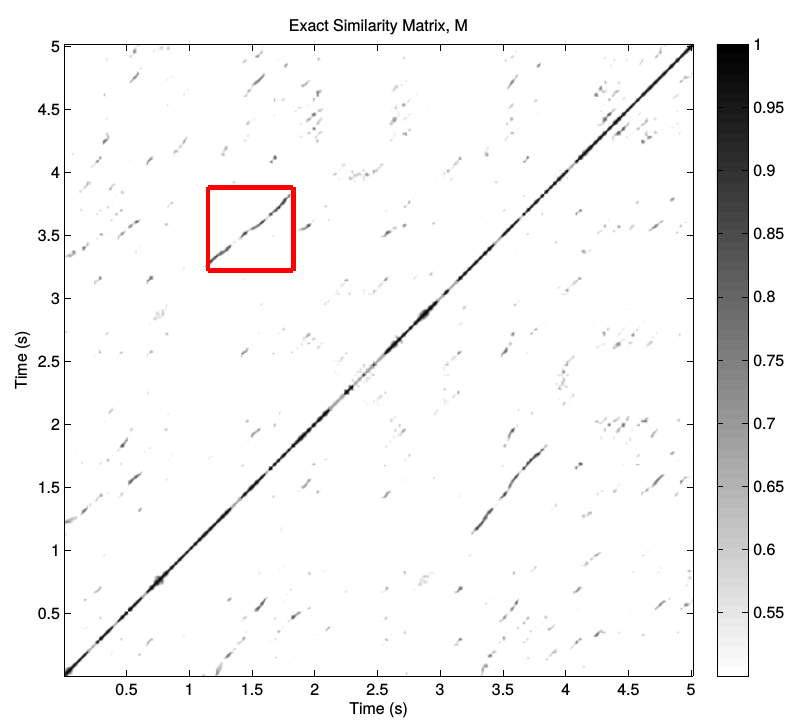
\includegraphics[width=4.5cm]{figures/similarity-matrix.png}

    \note[item]{Search for reoccurring patterns (e.g. words) in the audio}
    \note[item]{A dynamic time warping-based method is used here}
    \note[item]{Found patterns are aligned on a frame level to generate the frame pairs}
  \end{frame}
  
  \section{Method}
  \subsection{Motivation}
  
  \begin{frame}
    \frametitle{Proposed method -- motivation}
    
    \begin{itemize}
     \item Term discovery only covers a fraction of the data
     \begin{itemize}
      \item Would like to make more efficient use of all data
     \end{itemize}
     \item Large neural networks are prone to overfitting and difficult to interpret
     \item Idea: Use the whole data to find representations that are speaker dependent, but that can be used with simpler models
     \item Use a term discovery data to make these representations more speaker invariant
    \end{itemize}
  \end{frame}
  
  \subsection{Method description}
  \begin{frame}
    \frametitle{Proposed method}
    
    \begin{itemize}
     \item<1-> Infer a probabilistic model from the whole data
     \item<2-> The model will find speaker-dependent phonetic classes
     \item<3-> Use same-class and different-class frame pairs to merge the phonetic classes
     \item<4-> The classes are described using probabilities → merging is simple addition
    \end{itemize}
    
    \centering
    \begin{tikzpicture}[outpos/.style={draw,rectangle,onslide=<1-3>{text opacity=0}},
    inpos/.style={draw,circle,thick,onslide=<1>{text opacity=0}},
    arr/.style={->,thick},yscale=0.6]
    \visible<3->{\node[outpos] at (0,0) {$\Sigma$};
    \node[outpos] (out3) at (0,1) {$\Sigma$};
    \node[outpos] at (0,2) {$\Sigma$};
    \node[outpos] (out2) at (0,3) {$\Sigma$};
    \node[outpos] (out1) at (0,4) {$\Sigma$};}
    
  \node[inpos,onslide=<2->{blue}] (a1) at (-4, 3.5) {a};
  \node[inpos,onslide=<2->{red}] (a2) at (-4.5, 0.5) {a};
  \node[inpos,onslide=<2->{blue}] (k1) at (-3.4, 1.8) {k};
  \node[inpos,onslide=<2->{red}] (k2) at (-2.5, 1.5) {k};
    \node[inpos] (k3) at (-2.5, 4.2) {k};
    \node[inpos] (m1) at (-1.8, 0.1) {m};
    
    \visible<3->{\draw (a1) edge[arr] (out2) (a2) edge[arr,bend right=24] (out2)
          (k1) edge[arr] (out1) (k2) edge[arr] (out1) (k3) edge[arr] (out1)
	  (m1) edge[arr] (out3);}
  \end{tikzpicture}
  
  \note[item]{corresponds to partition}
  \note[item]{stress unsupervised (both GMM training and merging)}
  \end{frame}
  
  \begin{frame}
    \frametitle{Proposed method (cont.)}
    
    \begin{itemize}
      \item Represent input as a probability vector $\mathbf x$
      \begin{itemize}
       \item Each element is the probability of a latent class
      \end{itemize} \pause
      \item Merging the classes is done using a linear transform: $\mathbf x \mathbf W$ \pause
      \uncover<1-3>{\item $\mathbf W$ describes a proper partitioning of the input iff:
      \begin{enumerate}
       \item Each element in $\mathbf W$ is either 0 or 1
       \item Each row in $\mathbf W$ contains exactly one 1
     \end{enumerate}} \pause
      \item We instead constrain $\mathbf W$ as follows:
      \begin{enumerate}
       \item Each element is positive
       \item Each row sums to 1
      \end{enumerate}
      \item Output of the model is a lower-dimensional probability vector
    \end{itemize}
    
    \note[item]{Merge using siamese model}
    \note[item]{Difficult to optimise with these constraints}
  \end{frame}
  
  \begin{frame}
   \frametitle{Proposed method (cont.)}
    
   \centering
   \tikz \pic{siamese};
   
   \note[item]{just to recap...}
    \note[item]{Siamese model needs to compare output similarity}
  \end{frame}


  \begin{frame}
    \frametitle{Loss function}
    
    \begin{itemize}
     \item The output is a probability vector
     \item We can measure similarity using a statistical divergence measure \pause
     \item Here: The root Jensen-Shannon divergence
    \begin{equation*}
      L(\mathbf W; \mathbf x, \mathbf y) = \sqrt{JS(\mathbf x \mathbf W || \mathbf y \mathbf W)}
    \end{equation*}
     \item Minimize if $\mathbf x$ and $\mathbf y$ are the same speech sound; maximize otherwise \pause
     \item Need to balance same-class and different-class losses over a minibatch
    \end{itemize}
  \end{frame}

  \begin{frame}
    \frametitle{Entropy penalty for encouraging sparsity}
    
    \begin{itemize}
     \item Merging corresponds to partitioning the speaker-dependent classes
     \item However, $\mathbf W$ as defined is not a proper partitioning \pause
     \item Using an entropy penalty on the model output we can encourage $\mathbf W$ to be an approximate partitioning
     
     \begin{equation*}
      L_H(\mathbf W; \mathbf x, \mathbf y) = H(\mathbf x \mathbf W) + H(\mathbf y \mathbf W)
     \end{equation*}
     \item Prevents the probability mass from being spread out over multiple outputs
     \item Implicitly makes the model sparse
    \end{itemize}

    \note[item]{recall constraints---forcing sparsity will cause row to contain single 1}
    \note[item]{penalty term, added to loss function}
    \note[item]{must be sparse to avoid spreading probability mass from single input}
  \end{frame}
  
  \begin{frame}
   \frametitle{Discretisation}
   
   \begin{itemize}
    \item The trained model can be discretised
    \item Set largest element on each row to 1
    \item Set all other elements to 0
    \item Yields a proper partitioning
   \end{itemize}
  \end{frame}

  
  \subsection{Illustration}
  
  \begin{frame}
    \frametitle{Spectrogram features}
   \centering
   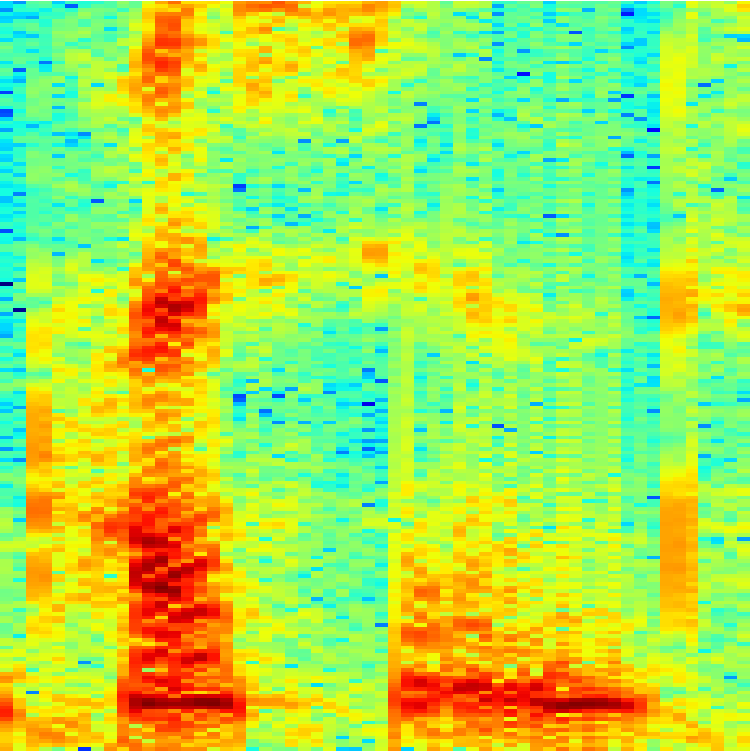
\includegraphics[width=6cm]{../report/data/spectrum-speaker-1-crop}
  \end{frame}
  
  \begin{frame}
    \frametitle{GMM features (input)}
   \centering
   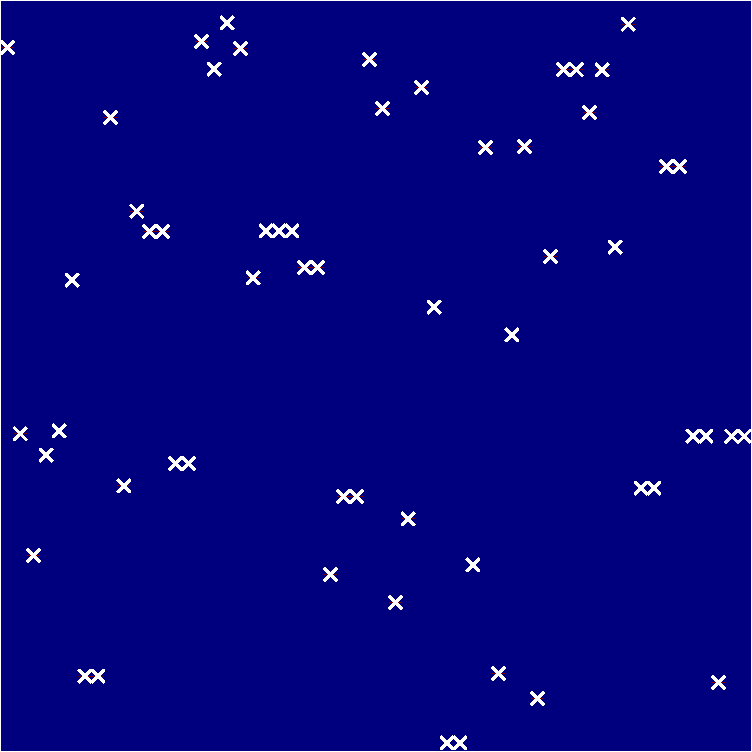
\includegraphics[width=6cm]{../report/data/gmm-posteriorgrams-speaker-1-crop}
  \end{frame}
  
  \begin{frame}
    \frametitle{Merged GMM features (output)}
   \centering
   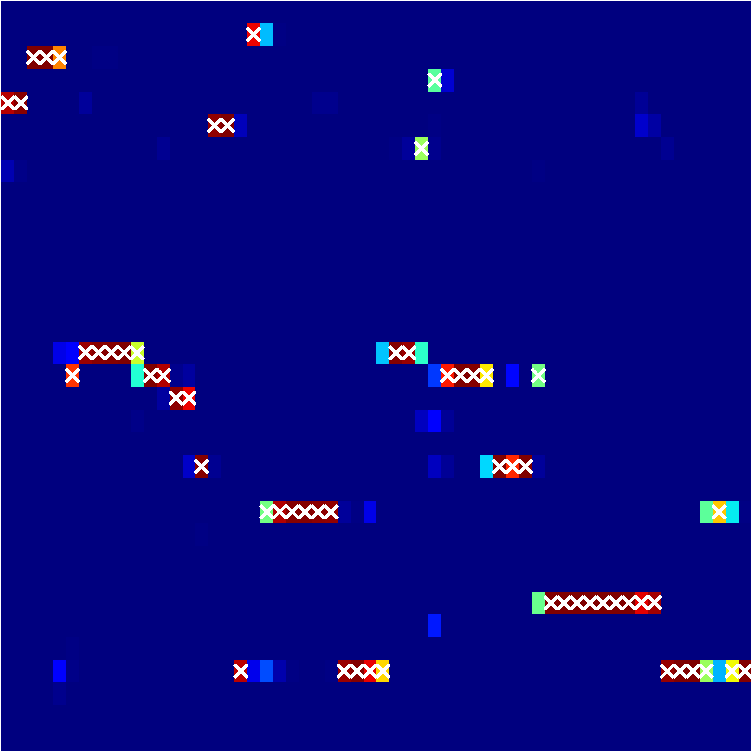
\includegraphics[width=6cm]{../report/data/reduced-posteriorgrams-speaker-1-crop}
  \end{frame}

  \section{Experiments}
  \subsection{Evaluation}
  \begin{frame}
    \frametitle{Data}
    
    \begin{itemize}
     \item Two corpora: One of casual English, and one of read Xitsonga
     \item The data is clustured using 1024-component GMMs
     \item For each frame we extract posterior probabilities from the GMM
     \item The proposed model is trained with 64 outputs
    \end{itemize}
    
    \note[item]{Bantu language spoken in southern Africa}
    \note[item]{for each corpus...}
    \note[item]{using frame pairs generated using term discovery}
  \end{frame}

  
  \begin{frame}
    \frametitle{Minimal-pair ABX}
    
    \begin{itemize}
     \item The evaluation is done using the minimal-pair ABX task
     \item Three utterances: A, B and X
     \item Either A or B is the same category as X
     \item Representing frames using the output of the model, the utterance most similar to X is chosen
    \end{itemize}
  \end{frame}
  
  \begin{frame}
    \frametitle{Results}
    \centering
 \begin{tabular}{lrrrr} \toprule
   & \multicolumn{2}{c}{English} & \multicolumn{2}{c}{Xitsonga} \\ \cmidrule(lr){2-3} \cmidrule(lr){4-5}
    Model & Within & Across & Within & Across \\ \midrule
    GMM posteriors & 12.3 & 23.8 & 11.4 & 23.2 \\ \midrule
    Proposed model & 12.8 & 19.8 & 14.0 & 23.2 \\
    Binary $\mathbf W$ & 12.0 & 19.3 & 12.7 & 21.9 \\ \midrule
    ABnet \footfullcite{thiolliere2015hybrid} & 12.0 & 17.9 & 11.7 & 16.6 \\
    DPGMM + LDA \footfullcite{heck2016unsupervised} & 10.6 & 16.0 & 8.0 & 12.6 \\ \bottomrule
 \end{tabular}
  \end{frame}

  \subsection{Conclusions}
  \begin{frame}
    \frametitle{Discussion}
    
    \begin{itemize}
     \item The model significantly decreases the dimensionality of the input
     \item At the same time, it empirically improves the speaker invariance of the representation
     \item Worse performance for Xitsonga -- sensitive to dimensionality?
     \item The model has few parameters, making it fast to train and robust against overfitting
     \item Can use probability vectors from any model as input
    \end{itemize}
  \end{frame}
  
  \begin{frame}
    \frametitle{Future work}
    
    \begin{itemize}
     \item Other models for generating the probability vectors
     \item Alternative loss functions
    \end{itemize}
  \end{frame}
  
  \begin{frame}
   Thank you for listening!
  \end{frame}


  
  % representation learning (not full solution)
  % talk about frames? feature vectors
  % ABnet - UTD, siamese
  % discuss method: UTD, GMM, siamese (shallow)
  % entropy penalty - enforce sparsity
  % ABX (discuss earlier?)
  % results

\end{document}
